La conception d'un système d'intelligence artificielle conversationnel robuste ne peut se faire sans une compréhension fine des paradigmes existants. Ce chapitre analyse l'évolution des architectures de \gls{nlp} pour justifier la transition vers une approche hybride, avant de détailler le cadre méthodologique et technique mis en œuvre.

\section{État de l'art}

Le domaine des agents conversationnels a traversé trois phases d'évolution majeures, chacune tentant de repousser les limites cognitives de la précédente.

\subsection{Approche Symbolique et Déterministe}
Historiquement, les premiers systèmes reposaient sur des règles manuelles (systèmes experts) ou des arbres de décision statiques. L'introduction du \gls{nlu} a permis de classifier les intentions utilisateurs avec plus de souplesse, mais la gestion du dialogue restait confinée à des scénarios pré-écrits. Ces systèmes garantissent une réponse contrôlée mais manquent de capacité de généralisation face à des requêtes inédites.

\subsection{L'Avènement du RAG Vectoriel}
La publication du papier "Attention Is All You Need" \cite{vaswani2017} a ouvert l'ère des Transformers et des \gls{llm}. Pour pallier le problème des connaissances figées et des hallucinations, l'architecture \gls{rag} (\textit{Retrieval-Augmented Generation}) a été théorisée par \cite{lewis2020}.

Le principe standard consiste à fragmenter (\gls{chunking}) les documents d'entreprise, à les convertir en vecteurs via un modèle d'\gls{embedding}, et à les stocker dans une \gls{vectordatabase} telle que PostgreSQL avec \textit{pgvector} \cite{pgvector}.
\begin{itemize}
    \item \textbf{Avantage :} Cette méthode permet d'ancrer le \gls{llm} dans une réalité documentaire privée.
    \item \textbf{Limite :} Comme le soulignent les travaux récents de Microsoft Research \cite{edge2024}, le RAG vectoriel souffre de "myopie". Il excelle dans la recherche de similarité de surface mais échoue à capturer les structures complexes ou les liens de causalité indirects (ex: A est compatible avec B, qui est un composant de C).
\end{itemize}

\subsection{L'Émergence du GraphRAG et la Convergence Neuro-Symbolique}
Pour surmonter ces limites, la recherche actuelle s'oriente vers l'intégration des \gls{knowledgegraph} dans les pipelines génératifs, une approche nommée \gls{graphrag} \cite{neo4j2024}. En structurant les connaissances sous forme de nœuds et de relations (conformément aux principes du \gls{websemantique} \cite{hogan2021}), on permet au système non plus de "chercher" des mots, mais de "raisonner" sur des concepts.

Cette architecture hybride combine la puissance statistique des \gls{llm} avec la rigueur logique des bases de graphes, offrant une précision supérieure pour les tâches de raisonnement multi-sauts (\textit{multi-hop reasoning}).

% --- PLACEHOLDER IMAGE : Comparatif RAG Vectoriel vs GraphRAG ---
\begin{figure}[h]
    \centering
     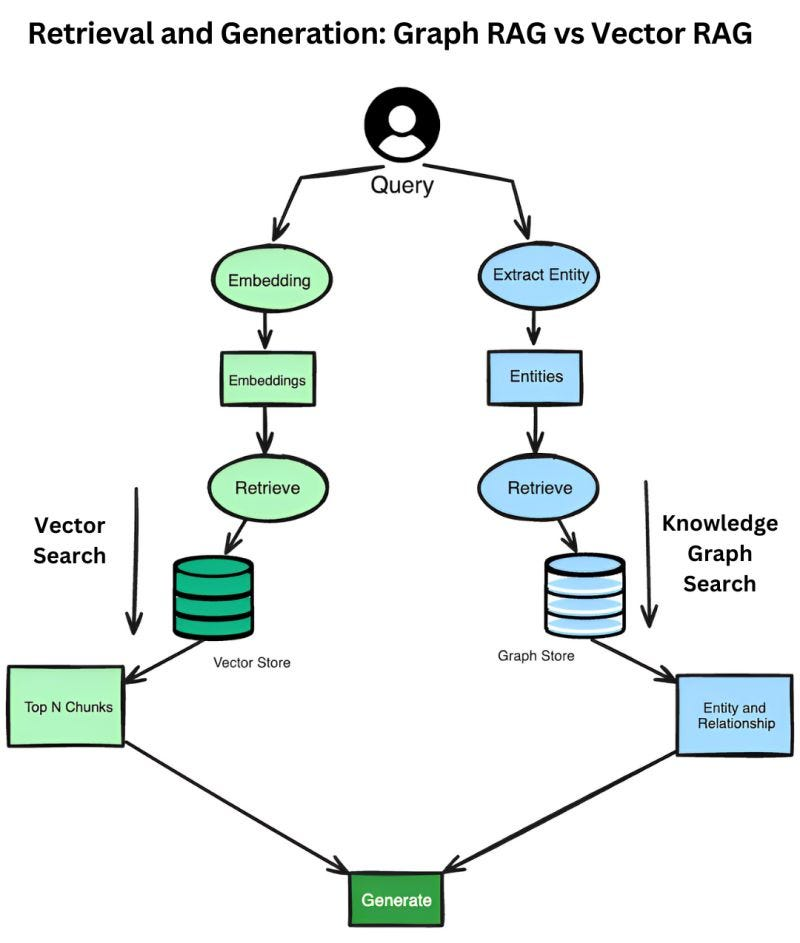
\includegraphics[width=0.4\textwidth]{docs/rag_vs_graphrag.jpg}
    \caption{Comparaison conceptuelle : La recherche par similarité (Vector) vs la traversée de relations (Graph). source \href{https://jillanisofttech.medium.com/which-rag-is-more-superior-graph-rag-or-vector-rag-55974f50b9c9}{jillanisofttech.medium.com/which-rag-is-more-superior-graph-rag-or-vector-rag-55974f50b9c9}}
    \label{fig:etat_art}
\end{figure}

\section{Méthodologie adoptée}

Compte tenu de la complexité inhérente à l'orchestration de ces technologies émergentes, nous avons adopté une méthodologie itérative et incrémentale de type \textbf{Agile Scrum}.

Le projet a été segmenté en \textbf{6 Sprints} intensifs, permettant une montée en complexité progressive :

\begin{enumerate}
    \item \textbf{Sprint 1 - Fondations NLU :} Mise en place de l'environnement de \gls{conteneurisation} (Docker) et développement d'un modèle Spacy pour la classification d'intentions transactionnelles simples.
    \item \textbf{Sprint 2 - RAG Vectoriel :} Implémentation du pipeline d'ingestion et connexion à la \gls{vectordatabase}. Cette phase a permis de valider le concept de récupération d'information contextuelle \cite{lewis2020}.
    \item \textbf{Sprint 3 - Interface Temps Réel :} Développement du Frontend Next.js et de la couche de communication asynchrone via \gls{websocket}.
    \item \textbf{Sprint 4 - Intelligence Émotionnelle :} Intégration de l'analyse de sentiment et du support multilingue (Arabe), préparant l'agent aux spécificités du marché cible.
    \item \textbf{Sprint 5 - Migration GraphRAG :} Pivot technologique majeur avec l'intégration de \gls{neo4j}. Utilisation d'un \gls{llm} pour extraire automatiquement les entités et relations, transformant le corpus non structuré en graphe \cite{edge2024}.
    \item \textbf{Sprint 6 - Consolidation \& Mémoire :} Ajout de la persistance contextuelle via \gls{redis} pour gérer les dialogues suivis et optimisation finale du \gls{promptengineering}.
\end{enumerate}

\section{Outils et Ressources}

L'écosystème technique a été sélectionné pour garantir performance, scalabilité et conformité aux standards de l'industrie.

\subsection{Stack Logicielle (Software)}
\begin{itemize}
    \item \textbf{Langage Principal :} Python 3.11 (Backend), choisi pour la richesse de son écosystème en IA et Data Science.
    \item \textbf{Framework Backend :} FastAPI, sélectionné pour sa performance en gestion asynchrone, indispensable pour l'\gls{orchestrateur} qui gère de multiples appels API parallèles.
    \item \textbf{Orchestration IA :} \gls{langchain} (v0.3+), utilisé pour chaîner les appels au \gls{llm} et gérer la conversion Texte-vers-Cypher \cite{langchain2024}.
    \item \textbf{Modèle de Langage :} Google Gemini 2.5 Flash \cite{google2024}, retenu pour sa fenêtre de contexte étendue et son coût optimisé par rapport à GPT-4.
\end{itemize}

\subsection{Infrastructure de Données (Data Stack)}
\begin{itemize}
    \item \textbf{Graphe :} \gls{neo4j} (Community Edition), le standard industriel pour le stockage de données hautement connectées.
    \item \textbf{Vecteur :} PostgreSQL étendu avec \textit{pgvector}, assurant le stockage hybride (relationnel et vectoriel).
    \item \textbf{Cache :} \gls{redis}, utilisé pour le stockage éphémère de l'historique de session, garantissant une latence minimale lors de la récupération du contexte.
\end{itemize}

% --- PLACEHOLDER IMAGE : Diagramme de Stack Technique ---
\begin{figure}[h]
    \centering
    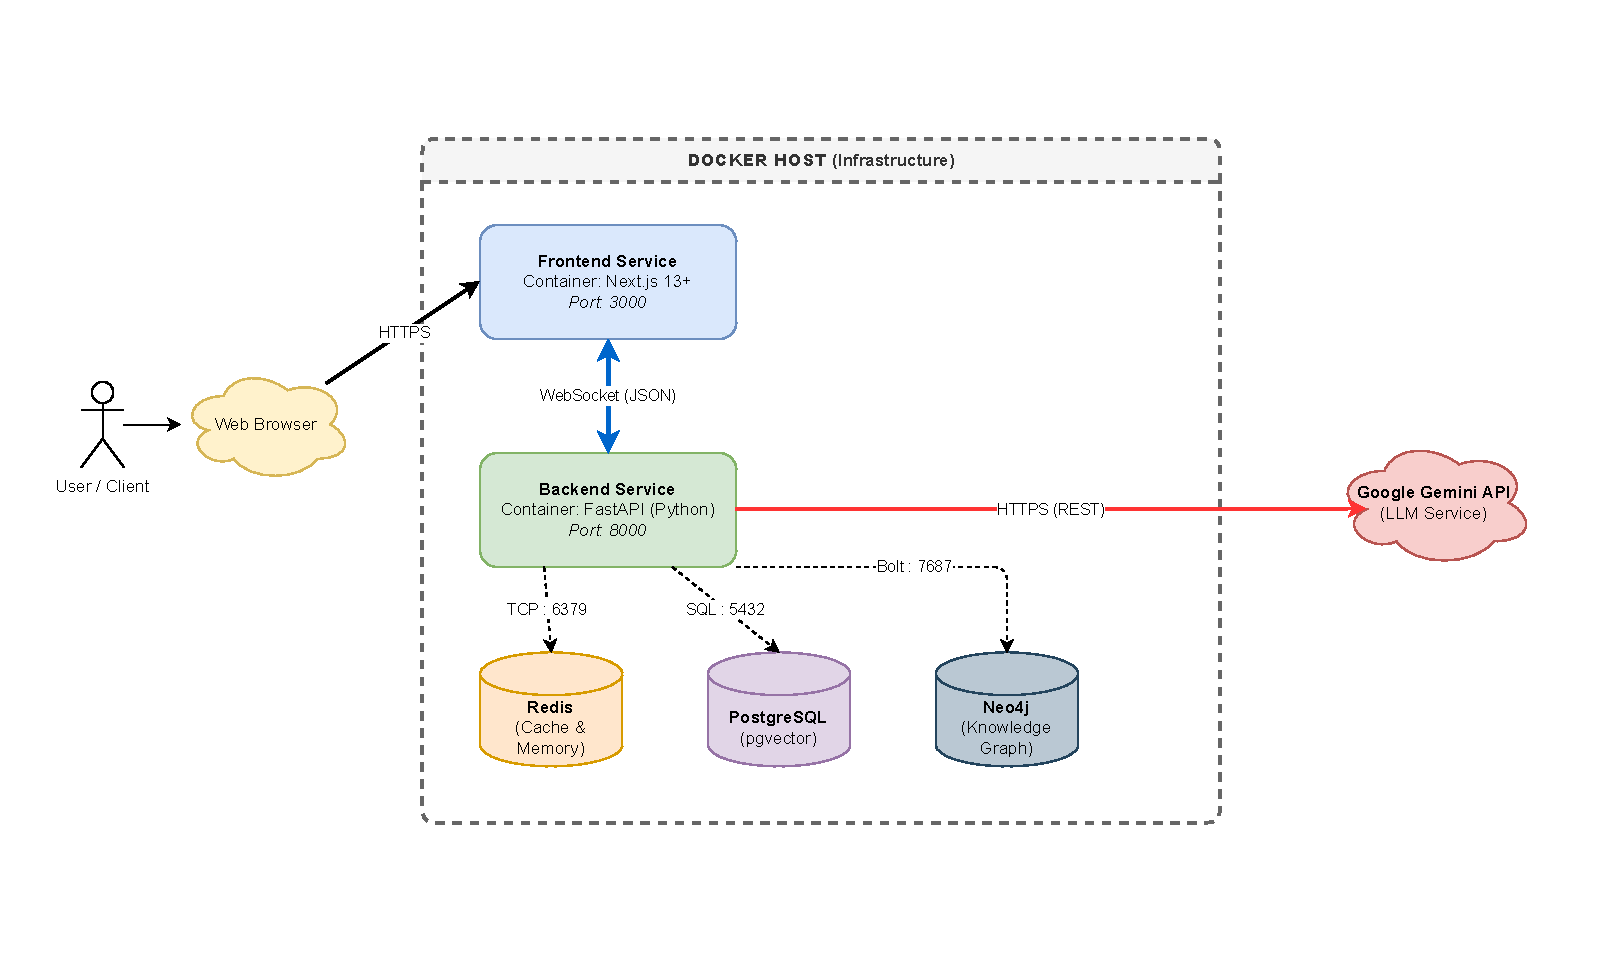
\includegraphics[width=1\textwidth]{docs/tech_stack.pdf}
    \caption{Vue d'ensemble de la Stack Technique et des flux de données.}
    \label{fig:stack}
\end{figure}